\documentclass{csc_assignment4}
\usepackage[utf8]{inputenc}
\usepackage[letterpaper, portrait, margin=1in]{geometry}
\usepackage{calc}  % arithmetic in length parameters
\usepackage{enumitem}  % more control over list formatting
\usepackage{fancyhdr}  % simpler headers and footers
\usepackage{lastpage}  % for last page number
\usepackage{relsize}  % easier font size changes
\usepackage[normalem]{ulem}  % smarter underlining
\usepackage{url}  % verb-like typesetting of URLs
\usepackage{xfrac}  % nicer looking simple fractions for text and math
\usepackage{amsmath}
\usepackage{amssymb}
\usepackage{tikz}
\usepackage{algorithm}
\usepackage{algorithmic}
\usepackage{graphicx}
\usepackage{listings}
\graphicspath{{/}}
\usepackage[export]{adjustbox}
\usepackage{enumitem}
\usepackage{subcaption}
\usepackage{esvect}
\lstset{breaklines=true}

% ----------------------------------------------------------------
% TODO: Enter the assignment number, your name, and your student number below
% ----------------------------------------------------------------
\AssignmentName{Assignment 4}
\StudentName{Akhil Gupta}
\StudentNumber{1000357071}

% ----------------------------------------------------------------
\begin{document}
\begin{description}

\item[Q1.]
\begin{enumerate}[label=(\alph*)]
\item How to compute disparity for a pair of parallel stereo cameras:\\ The formula for disparity as given in Professor Sanja's lecture slides is $x_{l} - x_{r}$ where $x_{l}$ and $x_{r}$ are the left and right image points on the left and right parallel cameras' image planes respectively. Then, in order to compute depth $Z$, we use $Z = \cfrac{f . T}{x_{l} - x_{r}}$ where $f$ is the focal length of the camera, $T$ is the baseline value. Both these can be determined from the camera instrinsic parameters matrix. 
\item How to compute the fundamental matrix from a pair of uncalibrated (non-parallel) cameras:\\ The fundamental matrix $F$ is a 3x3 matrix and is defined as $I_{r} = Fp_{l}$ where $I_{r}$ is the right epipolar line corresponding to the point $p_{l}$. $F$ has 9 elements but since we do not care about scaling, it only has 8 elements and we can effectively estimate $F$ with only 7 pairs of matching points in both images. To compute $F$, we need to solve: where $f$ is 3x3 where $n \ge 7$
\[
  \vv{f}
  \begin{bmatrix}
	x_{r, 1}x_{l, 1} & x_{r, 1}y_{l, 1} & x_{r, 1} & y_{r,1}x_{l,1} & y_{r,1}y_{l,1} & y_{r,1} & x_{l,1} & y_{l,1} & 1\\
	& & & & . & & &\\
	& & & & . & & &\\
	& & & & . & & &\\
	x_{r, n}x_{l, n} & x_{r, n}y_{l, n} & x_{r, n} & y_{r,n}x_{l,n} & y_{r,n}y_{l,n} & y_{r,n} & x_{l,n} & y_{l,n} & 1
  \end{bmatrix}
  = 0
\]
To use $F$ for the stereo problem, we can compute homographies that transform each image plane sich that they are parallel and since we can easily solve stereo for parallel cameras, we can proceed as usual. 
\item Compute depth of first 3 images (I used the same code just changed the imread file path for each image): \\
\begin{lstlisting}[language=MATLAB]
K =  [[721.5377,    0, 609.5593],
      [  0,  721.5377, 172.8540],
      [  0,    0,  1.0000]];
  
baseline = 0.5327;
img = imread('data/test/left/005002.jpg');
disp = imread('data/test/results/005002_left_disparity.png');
disparity = double(disp)/256;

Z = (721.5377*baseline)./(disparity);

i = 1;
for r = 1:size(Z, 1)
    for c = 1:size(Z, 2)
        xyz(i, :) = (K \ [c-1 ; r-1; 1])' * Z(r,c);
        i = i + 1;
    end
end

X = xyz(:,1);
Y = xyz(:,2);
Z = xyz(:,3);

surf(xyz, img, 'FaceColor', 'texturemap', 'EdgeColor', 'none')
view(0, 1000)
\end{lstlisting}
\begin{figure}[h]
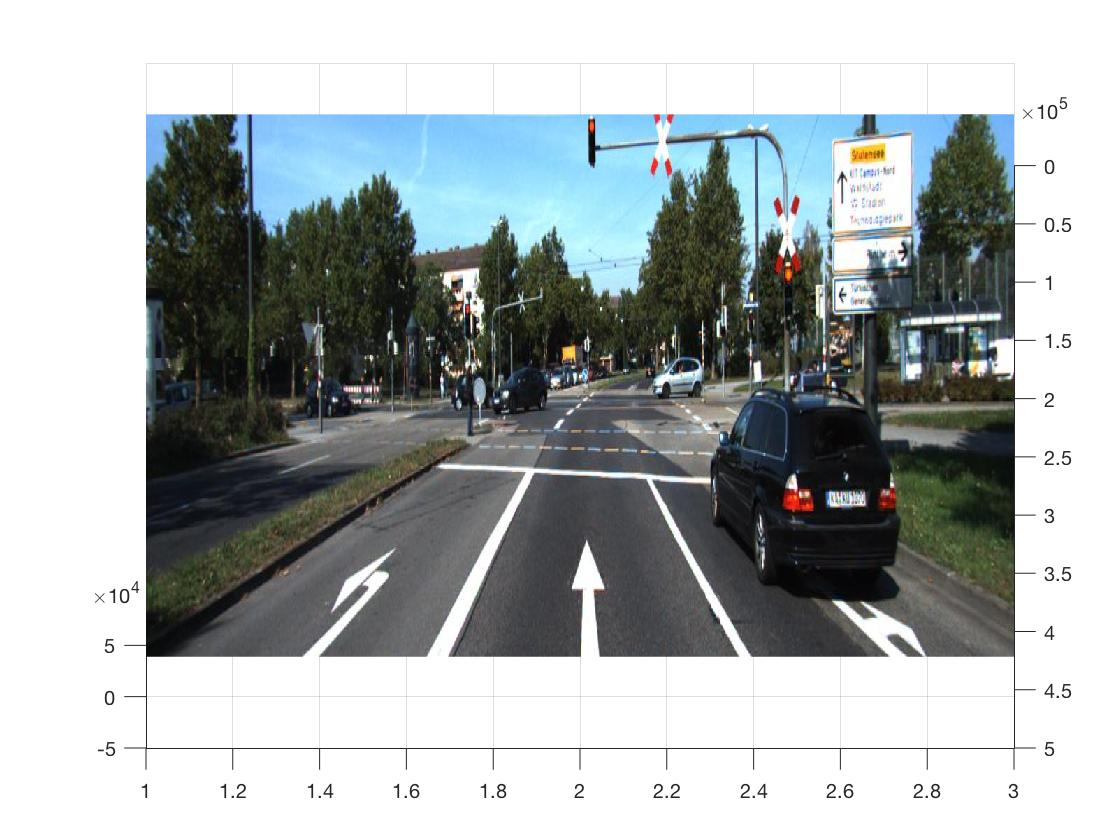
\includegraphics[width=1.0\textwidth, center]{data/a4q1c/004945_depth.jpg}
\vspace*{-5mm}
\caption{004945 depth rotated}
\end{figure}
\begin{figure}
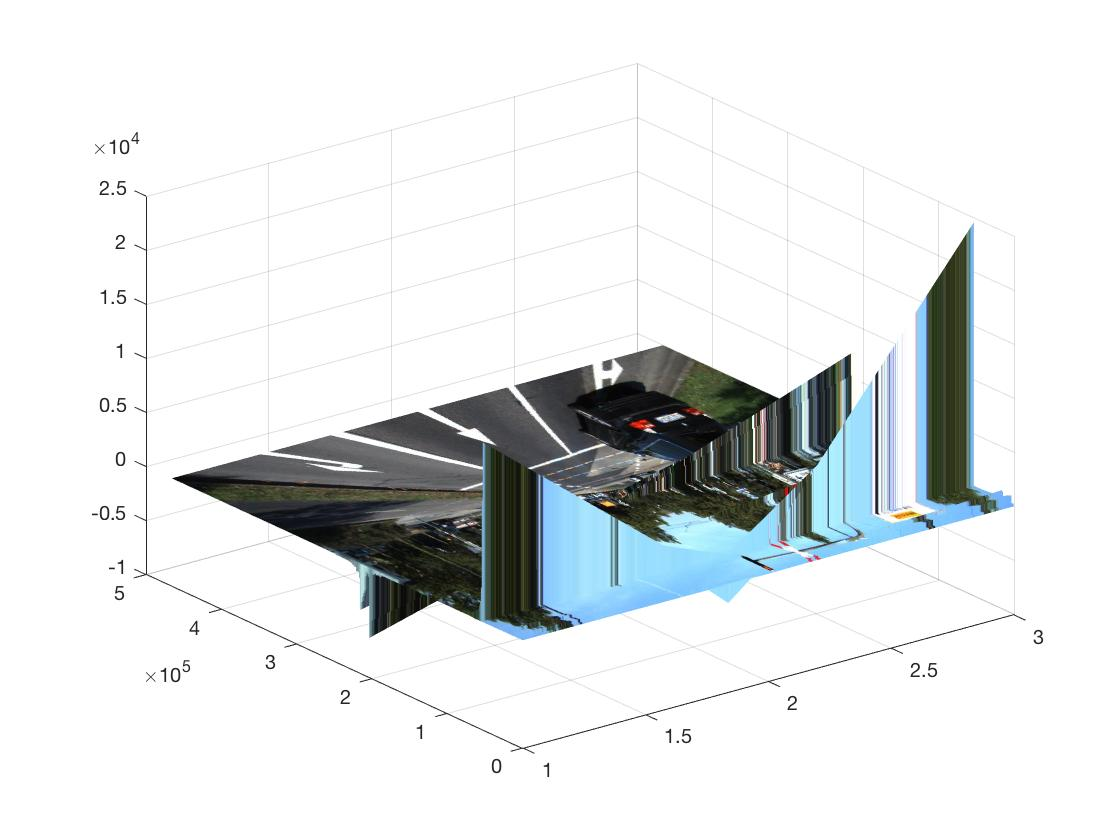
\includegraphics[width=0.8\textwidth, center]{data/a4q1c/004945_depth_rotated.jpg}
\vspace*{-5mm}
\caption{004945 depth}
\end{figure}
\begin{figure}
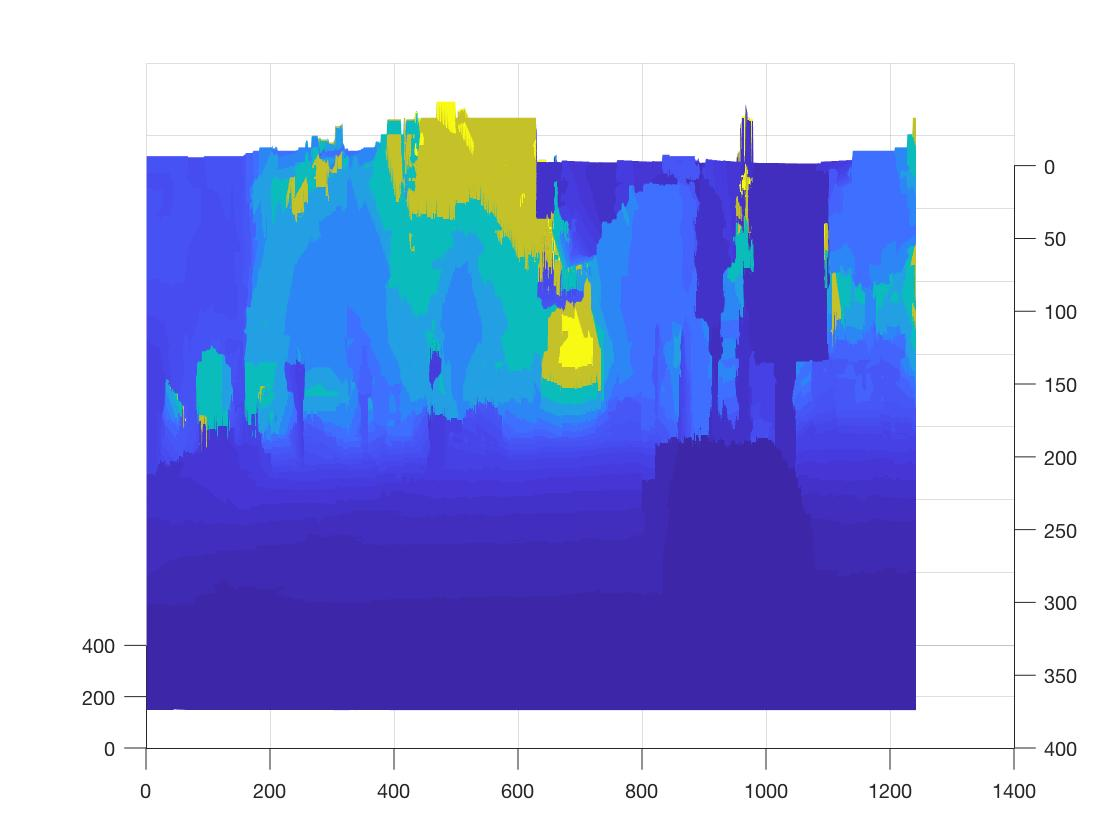
\includegraphics[width=0.8\textwidth, center]{data/a4q1c/004945.jpg}
\vspace*{-5mm}
\caption{004945 depth matrix}
\end{figure}
\begin{figure}
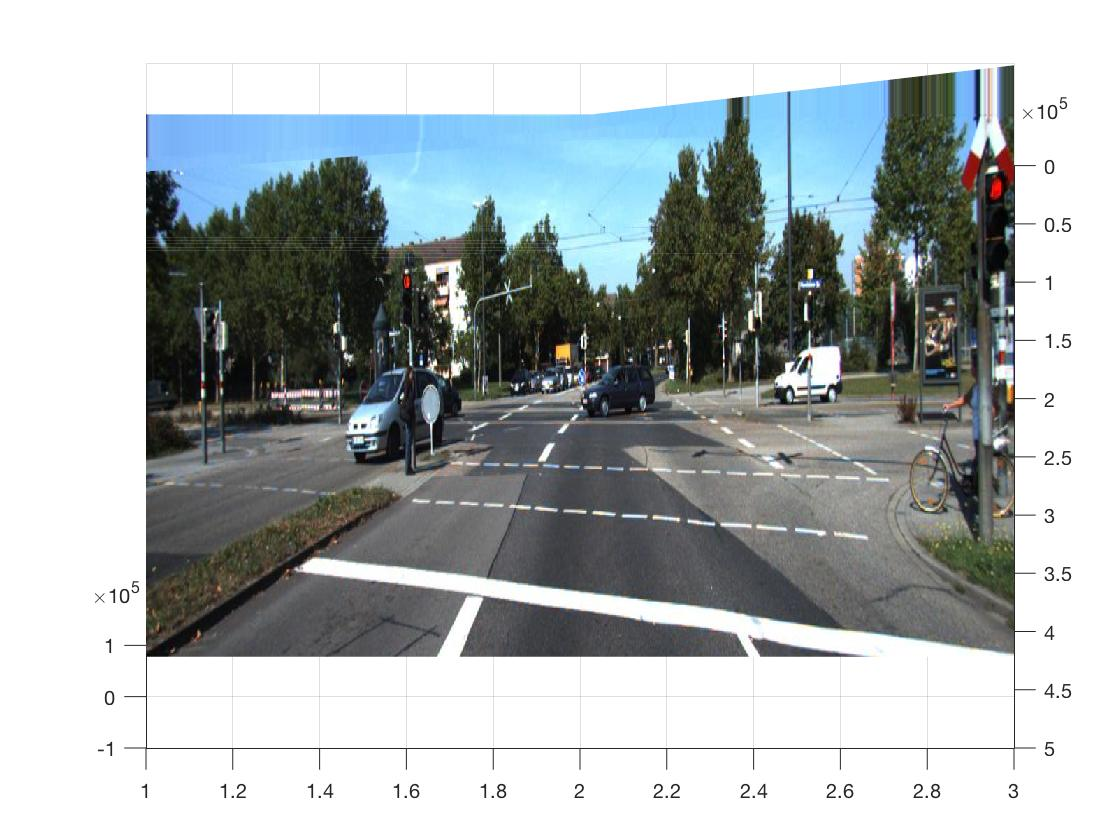
\includegraphics[width=0.8\textwidth, center]{data/a4q1c/004964_depth.jpg}
\vspace*{-5mm}
\caption{004964 depth rotated}
\end{figure}
\begin{figure}
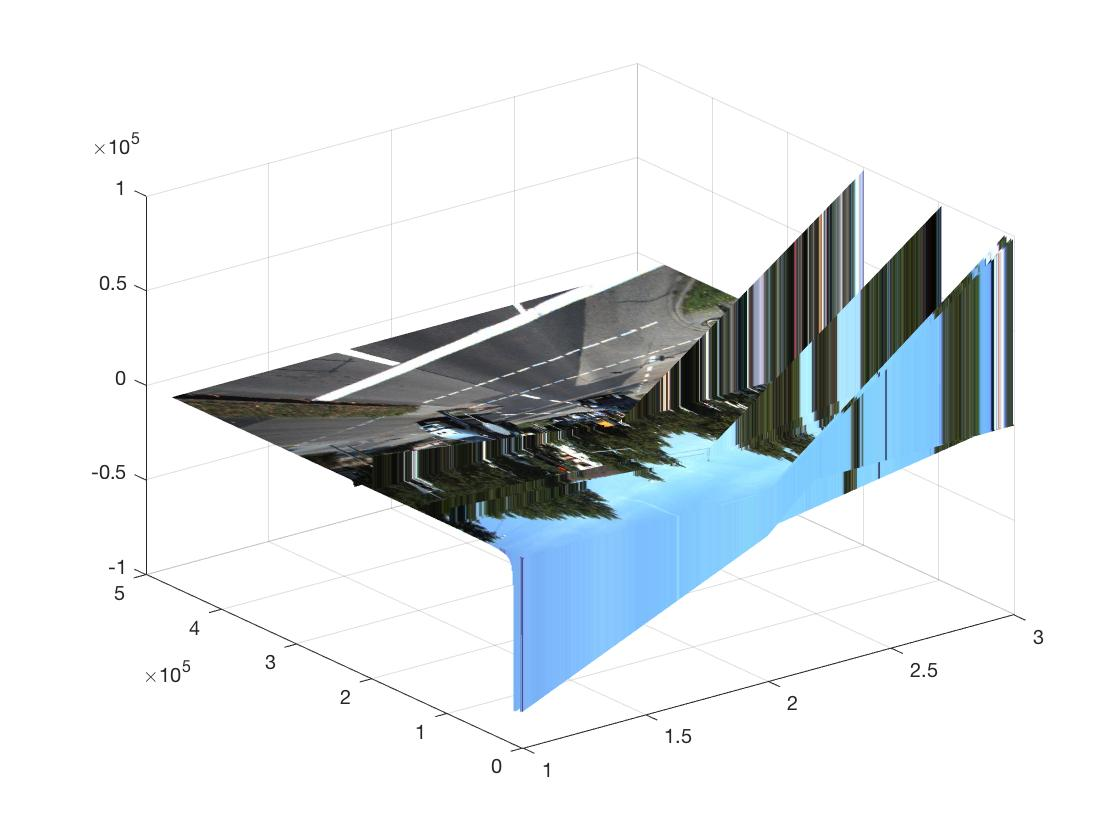
\includegraphics[width=0.8\textwidth, center]{data/a4q1c/004964_depth_rotated.jpg}
\vspace*{-5mm}
\caption{004964 depth}
\end{figure}
\begin{figure}
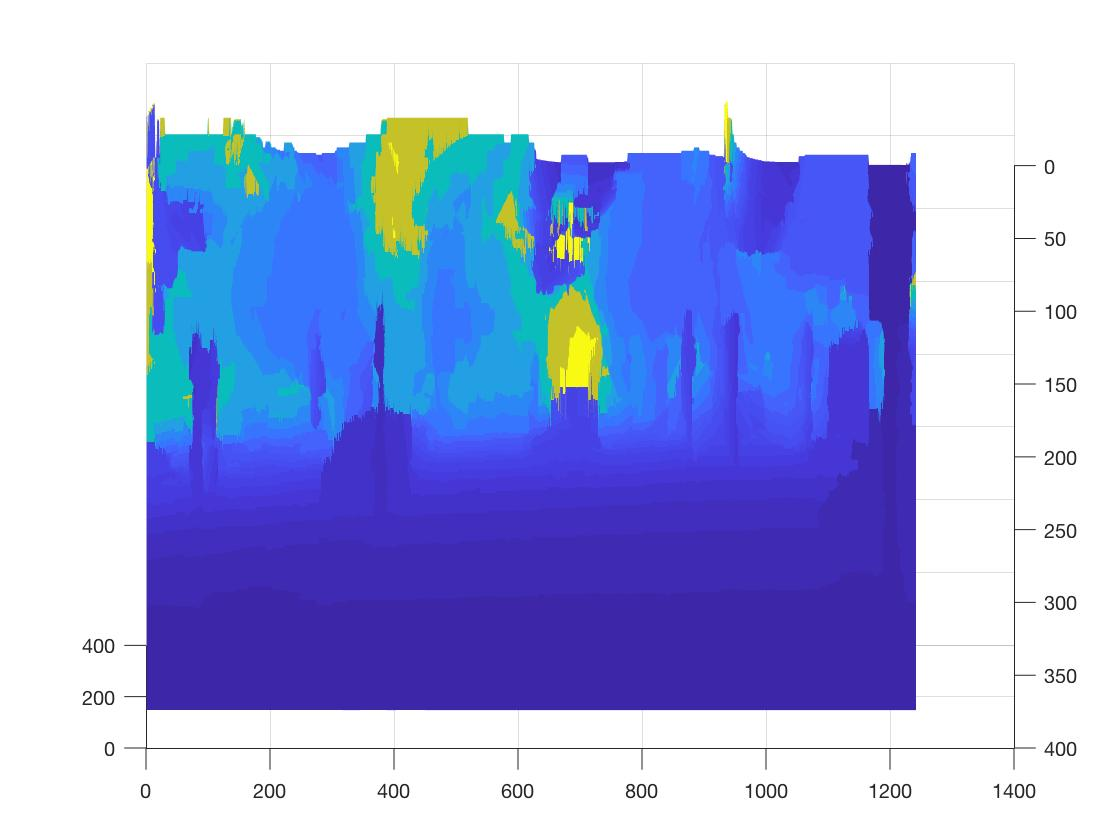
\includegraphics[width=0.8\textwidth, center]{data/a4q1c/004964.jpg}
\vspace*{-5mm}
\caption{004964 depth matrix}
\end{figure}
\begin{figure}
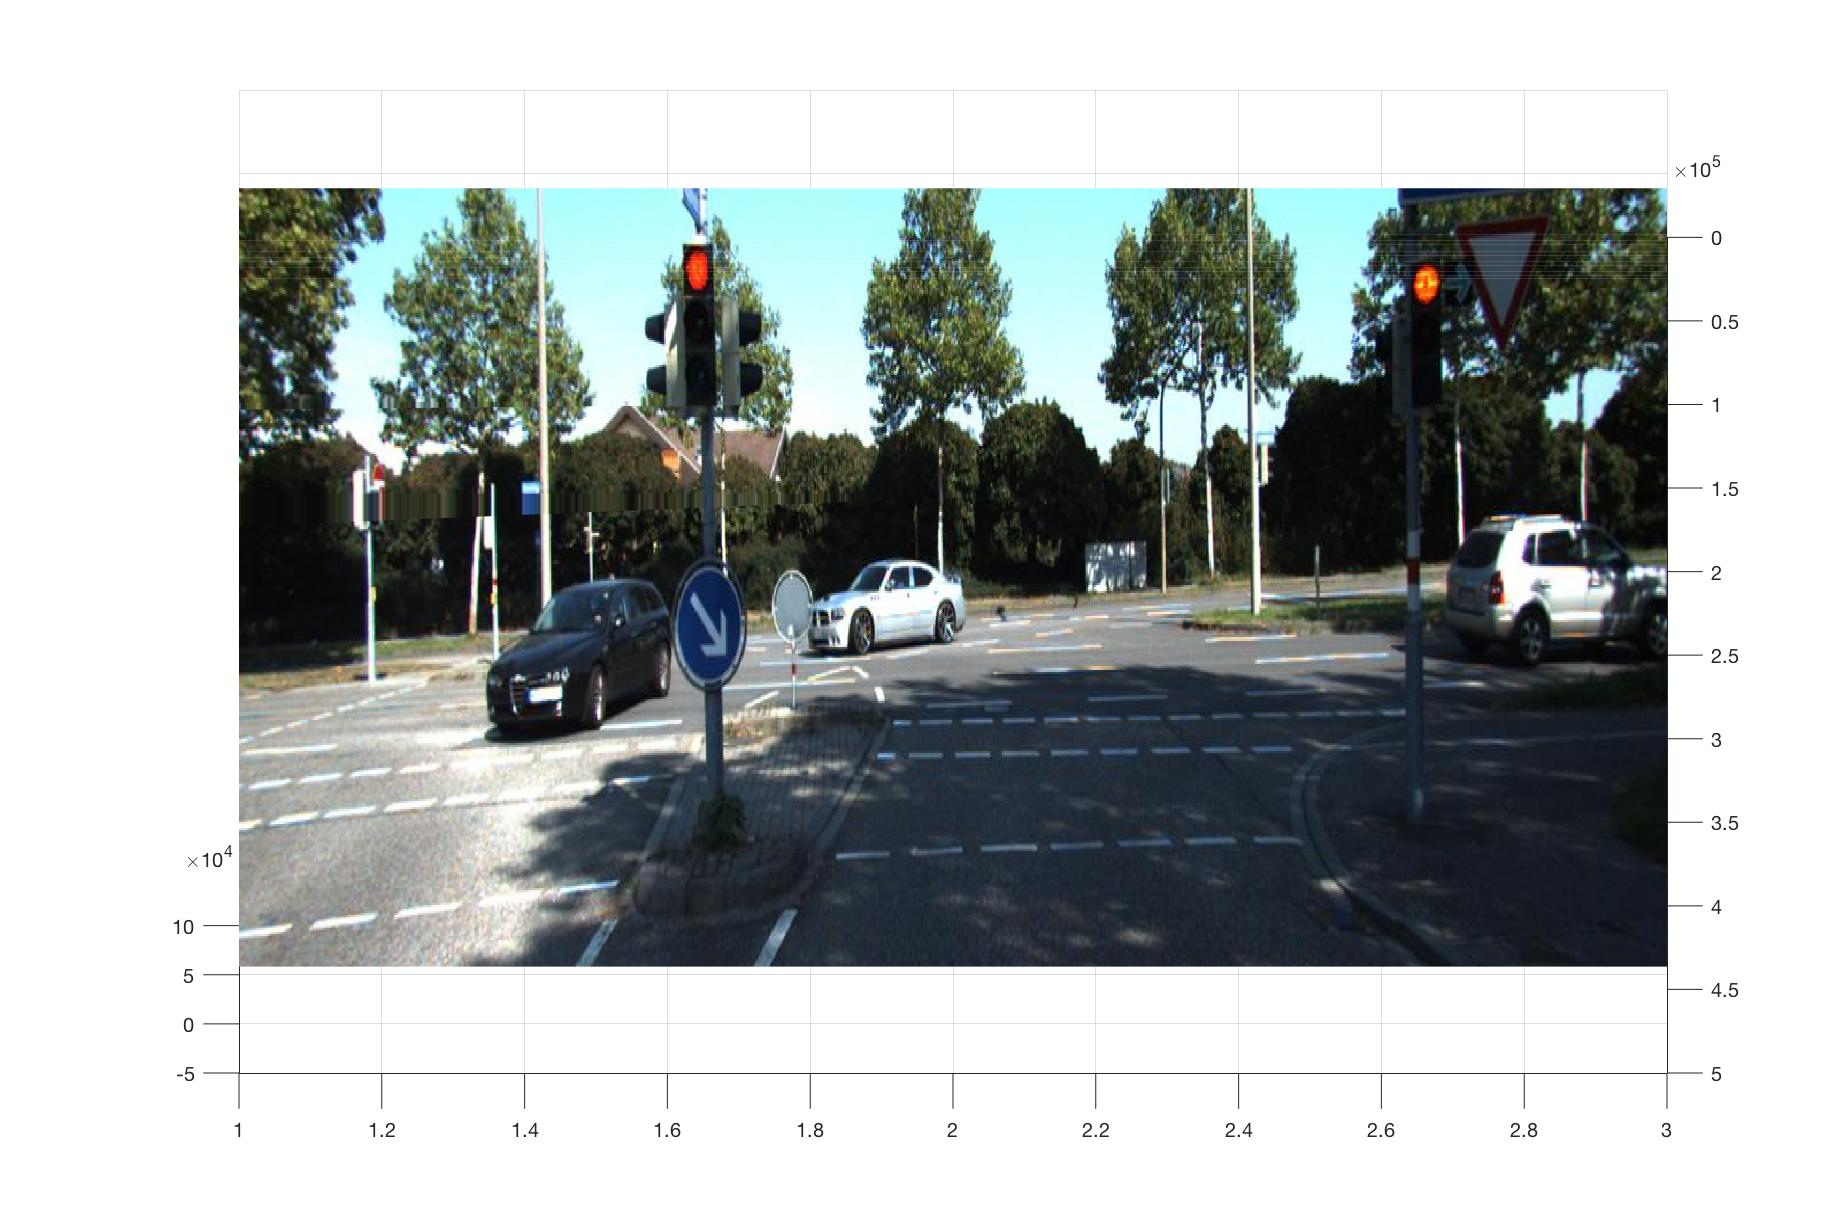
\includegraphics[width=0.8\textwidth, center]{data/a4q1c/005002_depth.jpg}
\vspace*{-5mm}
\caption{005002 depth rotated}
\end{figure}
\begin{figure}[t!]
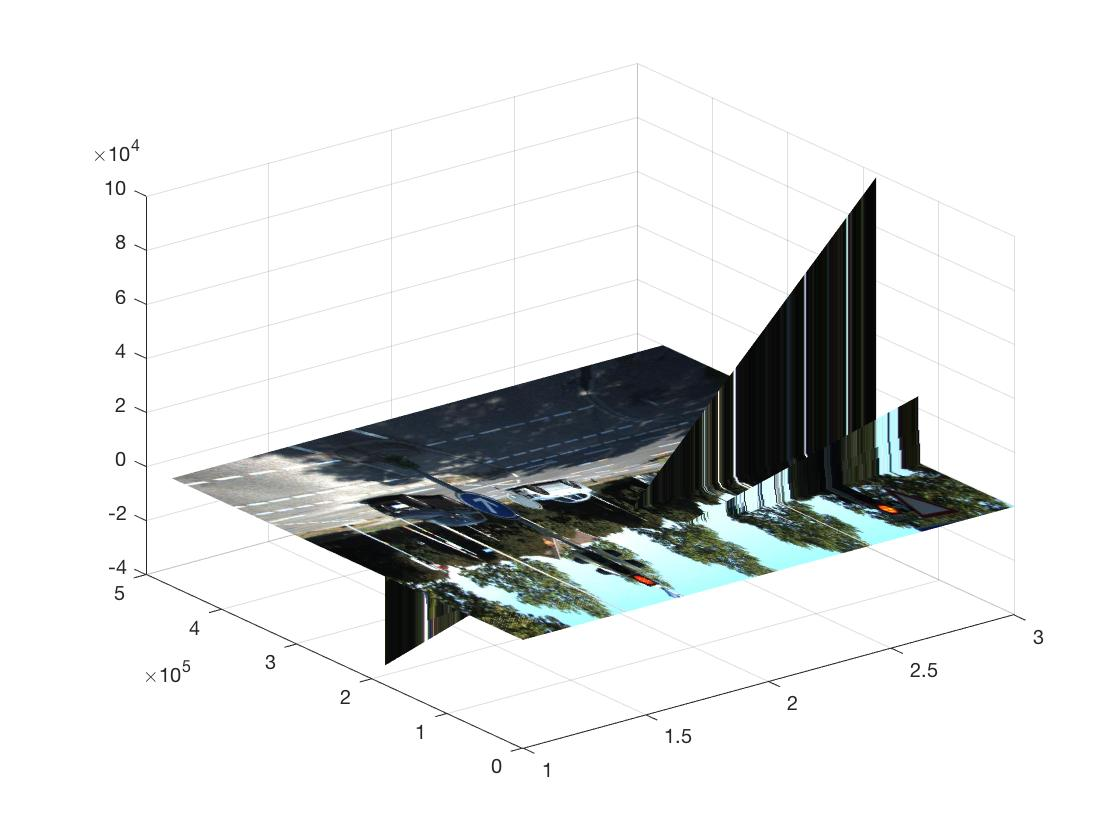
\includegraphics[width=0.8\textwidth, center]{data/a4q1c/005002_depth_rotated.jpg}
\vspace*{-5mm}
\caption{005002 depth}
\end{figure}
\begin{figure}
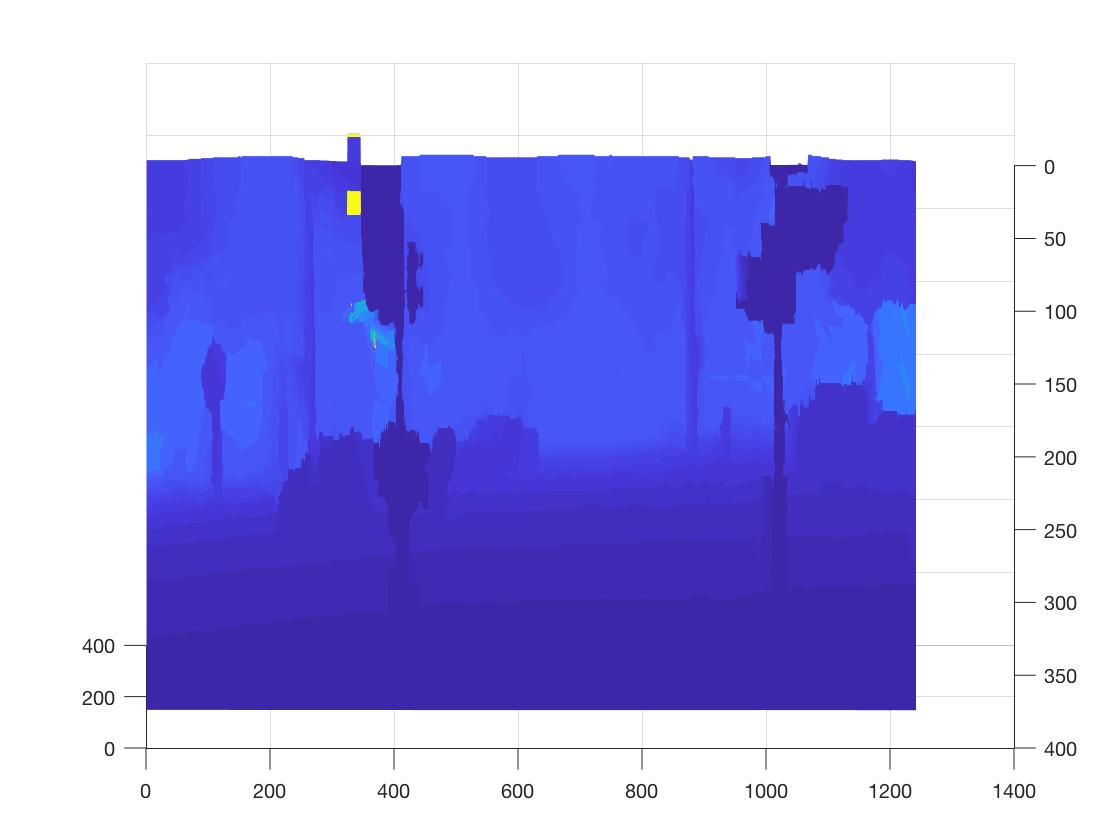
\includegraphics[width=0.8\textwidth, center]{data/a4q1c/005002.jpg}
\vspace*{-5mm}
\caption{005002 depth matrix}
\end{figure}

\clearpage
\item $[x_{left}, y_{top}, x_{right}, y_{bottom}, id, score]$
\item Visualization of car, person and cyclist detections
\begin{figure}[h!]
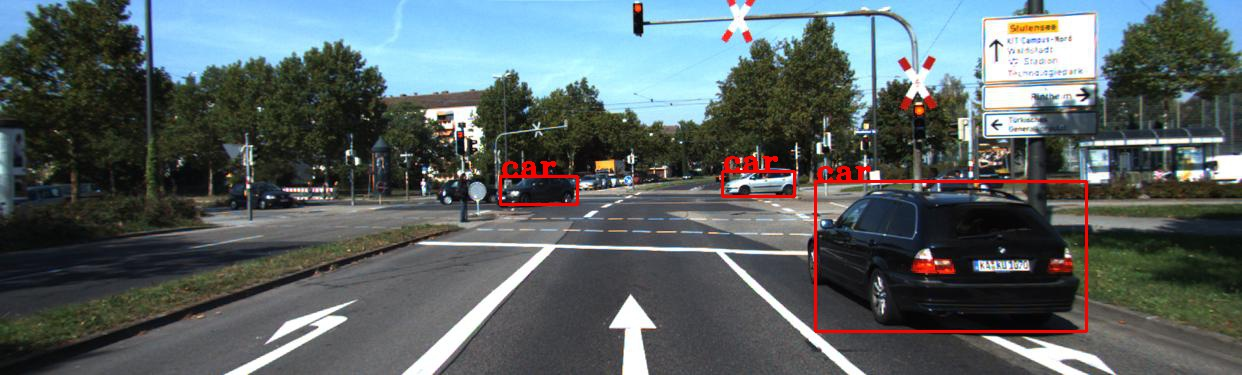
\includegraphics[width=1.0\textwidth, center]{code/004945.jpg}
\vspace*{-5mm}
\caption{004945}
\end{figure}
\begin{figure}[h!]
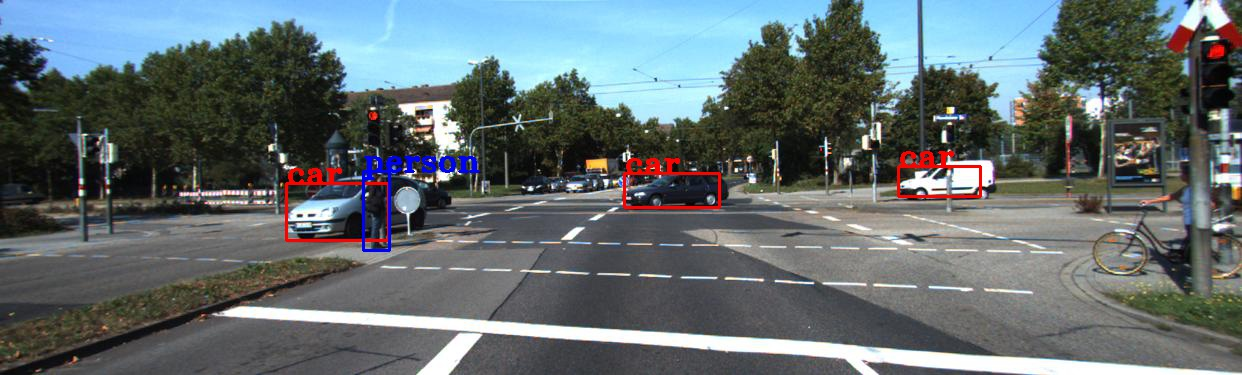
\includegraphics[width=1.0\textwidth, center]{code/004964.jpg}
\vspace*{-5mm}
\caption{004964}
\end{figure}
\begin{figure}[h!]
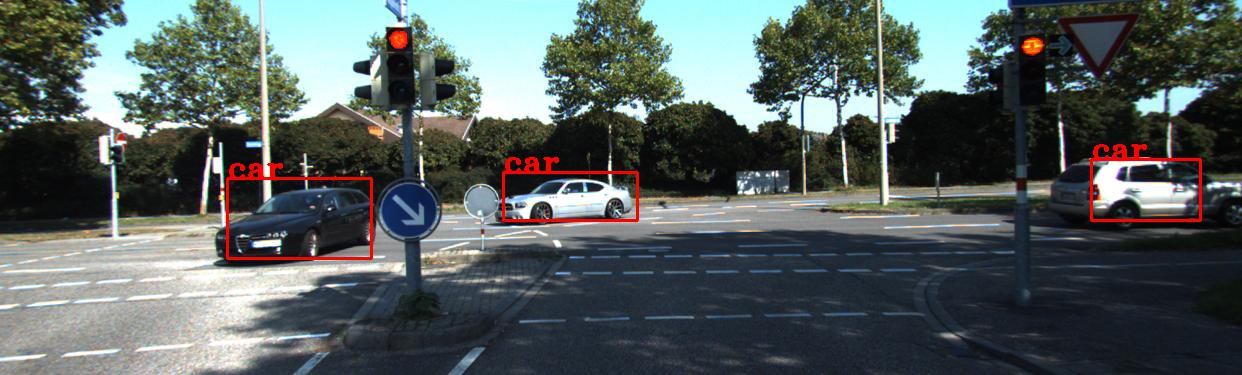
\includegraphics[width=1.0\textwidth, center]{code/005002.jpg}
\vspace*{-5mm}
\caption{005002}
\end{figure}

\newpage
\begin{lstlisting}[language=Python]
import cv2
import scipy.io as sci

font = cv2.FONT_HERSHEY_TRIPLEX
# Read input images
img1 = cv2.imread('../data/test/left/004945.jpg') # 3 cars
img2 = cv2.imread('../data/test/left/004964.jpg') # 3 cars 1 person
img3 = cv2.imread('../data/test/left/005002.jpg') # 3 cars

# Read input matrix dets
mat1 = sci.loadmat('../data/test/results/004945_dets.mat')
mat2 = sci.loadmat('../data/test/results/004964_dets.mat')
mat3 = sci.loadmat('../data/test/results/005002_dets.mat')

car1, car2, car3 = [], [], []
for index in range(len(mat1['dets'][0][0]) + 1):
    car1.append(int(mat1['dets'][0][0][0][index]))

for index in range(len(mat1['dets'][0][0]) + 1):
    car2.append(int(mat1['dets'][0][0][1][index]))

for index in range(len(mat1['dets'][0][0]) + 1):
    car3.append(int(mat1['dets'][0][0][2][index]))

cv2.rectangle(img1, (car1[0], car1[1]), (car1[2], car1[3]), (0, 0, 255), 2)
cv2.rectangle(img1, (car2[0], car2[1]), (car2[2], car2[3]), (0, 0, 255), 2)
cv2.rectangle(img1, (car3[0], car3[1]), (car3[2], car3[3]), (0, 0, 255), 2)
cv2.putText(img1, 'car', (car1[0], car1[1]), font, 1, (0, 0, 255), 2)
cv2.putText(img1, 'car', (car2[0], car2[1]), font, 1, (0, 0, 255), 2)
cv2.putText(img1, 'car', (car3[0], car3[1]), font, 1, (0, 0, 255), 2)

car1, car2, car3, person1 = [], [], [], []
for index in range(len(mat2['dets'][0][0]) + 1):
    car1.append(int(mat2['dets'][0][0][0][index]))

for index in range(len(mat2['dets'][0][0]) + 1):
    car2.append(int(mat2['dets'][0][0][1][index]))

for index in range(len(mat2['dets'][0][0]) + 1):
    car3.append(int(mat2['dets'][0][0][2][index]))

for index in range(len(mat2['dets'][1][0]) + 3):
    person1.append(int(mat2['dets'][1][0][0][index]))

cv2.rectangle(img2, (car1[0], car1[1]), (car1[2], car1[3]), (0, 0, 255), 2)
cv2.rectangle(img2, (car2[0], car2[1]), (car2[2], car2[3]), (0, 0, 255), 2)
cv2.rectangle(img2, (car3[0], car3[1]), (car3[2], car3[3]), (0, 0, 255), 2)
cv2.rectangle(img2, (person1[0], person1[1]), (person1[2], person1[3]), (255, 0, 0), 2)
cv2.putText(img2, 'car', (car1[0], car1[1]), font, 1, (0, 0, 255), 2)
cv2.putText(img2, 'car', (car2[0], car2[1]), font, 1, (0, 0, 255), 2)
cv2.putText(img2, 'car', (car3[0], car3[1]), font, 1, (0, 0, 255), 2)
cv2.putText(img2, 'person', (person1[0], person1[1]), font, 1, (255, 0, 0), 2)

car1, car2, car3 = [], [], []
for index in range(len(mat3['dets'][0][0]) + 1):
    car1.append(int(mat3['dets'][0][0][0][index]))

for index in range(len(mat3['dets'][0][0]) + 1):
    car2.append(int(mat3['dets'][0][0][1][index]))

for index in range(len(mat3['dets'][0][0]) + 1):
    car3.append(int(mat3['dets'][0][0][2][index]))

cv2.rectangle(img3, (car1[0], car1[1]), (car1[2], car1[3]), (0, 0, 255), 2)
cv2.rectangle(img3, (car2[0], car2[1]), (car2[2], car2[3]), (0, 0, 255), 2)
cv2.rectangle(img3, (car3[0], car3[1]), (car3[2], car3[3]), (0, 0, 255), 2)
cv2.putText(img3, 'car', (car1[0], car1[1]), font, 1, (0, 0, 255), 2)
cv2.putText(img3, 'car', (car2[0], car2[1]), font, 1, (0, 0, 255), 2)
cv2.putText(img3, 'car', (car3[0], car3[1]), font, 1, (0, 0, 255), 2)

cv2.imshow ('004945', img1)
cv2.imshow ('004964', img2)
cv2.imshow ('005002', img3)

cv2.imwrite('004945.jpg', img1)
cv2.imwrite('004964.jpg', img2)
cv2.imwrite('005002.jpg', img3)
cv2.waitKey()
\end{lstlisting}

\item In order to compute the 3D location of each detected object in the above images, we use the same algorithm as in A3 Q3 and A4 Q1c). The 3D location basically consists of $(X, Y, Z)$ coordinates. We have already computed $Z$ (depth) from the camera intrinsic parameter matrix $K$ and the disparity map. Hence, we can easily compute $X$ and $Y$ where
$X = \cfrac{(Z[y,x] * (x - p_{x}))}{f}$, where $x, y$ is a 2D point on the image and $p_{x}$ and $f$ are from $K$. Similarly, $Y = \cfrac{(Z[y,x] * (y - p_{y}))}{f}$. In our case, for $(x, y)$ we can use our 'dets\{1\}' to get $[x_{left}, y_{top}, x_{right}, y_{bottom}, id, score]$. Hence, we can compute the 3D location of each detected object above. We can use depth to help us refine our 2D segmentation by grouping pixels of similar depth together within the bounding box of the detected object. 
\end{enumerate}

\item[Q2.] 
Hough Voting for finding circles of known radius $r$ in an image:
\begin{enumerate}
\item We know that equation of a circle is $(x-a)^{2} + (y-b)^{2} = r^{2}$ where $(a,b)$ is the center of the circle and $r$ is the known radius. 
\item So in our 2D Hough space $(a,b)$: a sample point $(x_{0}, y_{0})$ maps to $(a-x_{0})^{2} + (b-y_{0})^{2} = r^{2}$ which is simply a circle centered at $(x_{0}, y_{0})$ with radius $r$.
\item Each point in the image space generates a circle in the Hough parameter space. The circles in the Hough space intersect at  $(a,b)$ which is the center in geometric space. 
\item So basically, we first load an image and detect edges (using Canny or something similar)\item Then for every 'edge' pixel, we generate a circle in the Hough space.
\item The intersection point of all such circles would be corresponding to the center of the original circle
\item If however, we do not know the radius $r$, we simply guess. We set $r$ = 1, 2, ..., length of the diagonal of the image because no circle will have a greater radius than the diagonal of the image. This leads to a 3D Hough space $(a, b, r)$ where each horizontal plane would be equal to the 2D parameter space when $r$ is known. 
\item Only, this time, instead of circles around our centers as in 2D Hough space, we end up with conics. We get a double cone around the centers of the circle. And the intersection of the 2 cones would be corresponding to the center of the original circle.
\end{enumerate}


\end{description}
\end{document}
  
  



